\documentclass[landscape,paperheight=24in,fontscale=.45,paperwidth=36in]{baposter}

\usepackage{blindtext}

\usepackage{amsmath}
\usepackage{amssymb}
\usepackage{amsfonts}
\usepackage{bbm}                     %% indicator function symbol

\usepackage{graphicx}
\usepackage{caption}                           %% custom captions
\usepackage{soul}                          %% colorful underlines

%% --- Define WZB color scheme ----------------------------------
\definecolor{wzbGreen}{cmyk}{0.366,0,0.967,0.4}
\definecolor{wzbBlue}{cmyk}{0.983,0.293,0,0.29}
\definecolor{wzbMagenta}{cmyk}{0,0.69,0.272,0.38}

%% --- define underline color -----------------------------------
\setulcolor{wzbBlue}

\begin{document}
\begin{poster}{
  % --- General options ------------------------------------
  eyecatcher=true,  %% No funny picture to left
  background=none, %% white background
  % --- Box header settings --------------------------------
  headershape=rounded, %% shape box header
  headerborder=open, %% add border to header
  headerColorOne=wzbBlue, %% bg color header
  headershade=plain, %% no color gradient header
  % --- Box settings ---------------------------------------
  boxshade=none, %% no color gradient box content
  borderColor=wzbBlue, %% border color box content
  textborder=roundedright %% bottom shape box border
}
{ % Worlmap displaying dictatorships in 2007
 \includegraphics[scale=.6]{/home/dag/Dropbox/Buero/Dissertation/2015/duke/classes/mle/termPaper/out/worldmapEyecatcher.pdf}
}
{\sf A dictator's toolkit. How cooptation affects repression in autocracies}
{
\textsf{Replicated by} Dag Tanneberg, Berlin Social Science Center,
  Dept. `Democracy and Democratization', dag.tanneberg@wzb.eu%
}
{

\includegraphics[scale=.5]{./quareise.png}
}
\headerbox{\sf \color{white} Summary}{name=summary,column=0,row=0}{
\begin{minipage}{\linewidth}
  \raggedright Frantz and Taylor explore the interaction of two instruments of 
  dictatorial rule: co-optation and political repression. They 
  find that co-optation in the form of political parties and 
  legislatures leads dictators to reduce restrictions on empowerment
  rights. Simultaneously it increases physical integrity violations
  as it draws opposition into the open. A closer look at the results
  provides evidence of notable model misspecification and weak 
  predictive power.
\end{minipage}
}

\headerbox{\sf \color{white} Method and Material}{name=methods,column=0,below=summary}{
  Ordered logistic regression: $\xi = \alpha + \boldsymbol{x}\boldsymbol{\beta}+\mathcal{\varepsilon}$
  \begin{align*}
    & y = \begin{cases}
      \text{level}~ 1 ~ \text{if} -\infty < \xi \le \alpha_1 \\
      \vdots \\
      \text{level}~ m-1 ~ \text{if} ~ \alpha_{m-2} < \xi \le \alpha_{m-1} \\
      \text{level}~ m ~ \text{if} ~ \alpha_{m-1} < \xi \le \infty \\
    \end{cases} \\
    & Pr(y \le j | \boldsymbol{x}) = Pr(\xi \le \alpha_j|\boldsymbol{x})
  \end{align*}
  Design: 138 dictatorships between 1972 and 2007 are analyzed 
  in a pooled cross-section design with 5 imputed datasets. The 
  study explores the effect of co-optation at $t$ on repression at
  $t+1$ to $t+5$.
}

\headerbox{\sf \color{white} First impression}{name=first,column=0,below=methods}{
  \begin{minipage}{\linewidth}
  \centering
  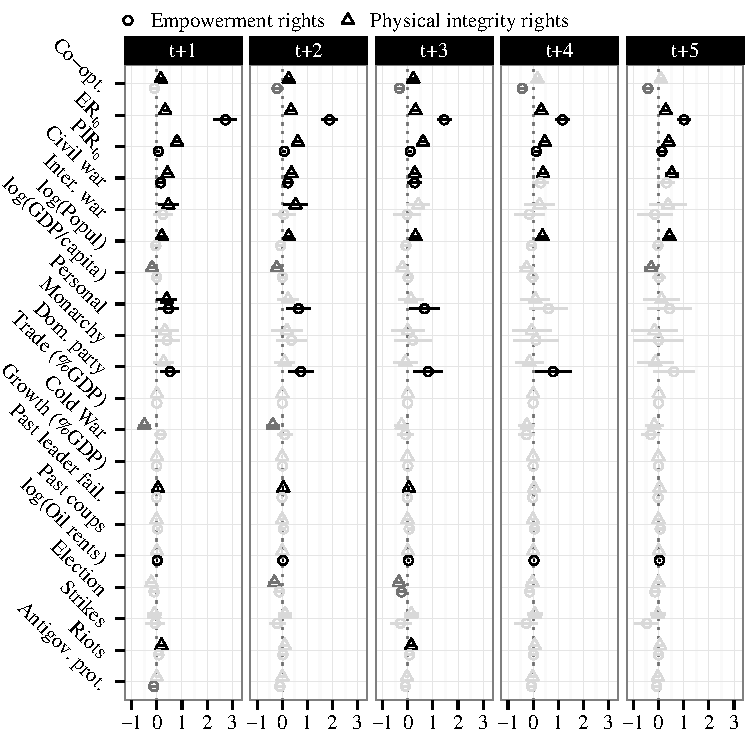
\includegraphics[width=3.6in]{/home/dag/Dropbox/Buero/Dissertation/2015/duke/classes/mle/termPaper/out/coefPlotOriginal.pdf} \\
  \raggedright
  The original results can be reproduced up to 2
  decimal places. Most often co-optation via 
  legislatures and political  parties {\color{wzbBlue} reduces} 
  restrictions on empowerment rights. Simultaneously, it 
  {\color{wzbMagenta} encourages} physical integrity violations.
  \end{minipage}
}
\headerbox{\sf \color{white} Replication results}{name=results,column=1,span=2,row=0,textborder=rounded,bottomaligned=first}{
\centering{\section*{\sf \underline{Parallel regressions assumption}}}
\begin{minipage}{.49\linewidth}
  \centering
  \includegraphics[width=3in]{/home/dag/Dropbox/Buero/Dissertation/2015/duke/classes/mle/termPaper/out/parallelRegrDevianceBonfP.pdf} \\
  \raggedright
  Using a $\chi^2$-test the coefficients from each imputation
  round can be compared to their multinomial alternatives. Only 
  four models reject the multinomial alternative hypothesis of 
  non-constant coefficients with average p-values above $0.05$.
\end{minipage}
\hfill
\begin{minipage}{.49\linewidth}
  \centering
  \includegraphics[width=3in]{/home/dag/Dropbox/Buero/Dissertation/2015/duke/classes/mle/termPaper/out/parallelRegressionsPosterPlot_ManualLabels.pdf} \\
  \raggedright
  An alternative test draws on $j-1$ logistic regressions with 
  response $\mathbbm{1}_y(y_{i} \ge j)$. Coefficients should differ 
  little as $j$ increases. Although perfect separation occurred 
  (not shown), the test raises strong concerns about co-optation.
\end{minipage}
\vfill
%% --- Separation plots -----------------------------------------
\begin{minipage}{.49\linewidth}
  \centering
  \section*{\sf \underline{Predictive accuracy}}
  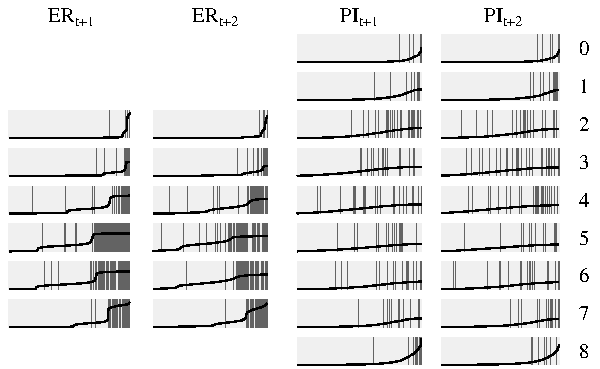
\includegraphics[width=3in]{/home/dag/Dropbox/Buero/Dissertation/2015/duke/classes/mle/termPaper/out/separation_revise.pdf} \\
  \raggedright
  As can be seen from the separation plots empowerment rights 
  restrictions at $t+1$ are somewhat reliably predicted.
  Already at $t+2$ predictive accuracy declines visibly. In 
  contrast, co-optation offers no leverage on physical integrity 
  violations.
\end{minipage}
\hfill
\begin{minipage}{.49\linewidth}
  \centering
  \section*{\sf \underline{Parsimony}}
  \includegraphics[width=3in]{/home/dag/Dropbox/Buero/Dissertation/2015/duke/classes/mle/termPaper/out/aicDifferences.pdf} \\
  \raggedright
  All models include lagged responses to account for serial 
  autocorrelation. However, in many cases the lagged response 
  offers the most parsimonious fit to the data. Again co-optation
  offers little leverage on political repression.
\end{minipage}
}
\headerbox{\sf \color{white} Future development}{name=development,column=3,row=0,textborder=roundedleft}{
  \blindtext
}
\headerbox{\sf \color{white} Conclusions}{name=conclusions,column=3,,textborder=roundedleft, below=development}{
  \blindtext[1]
}
\headerbox{\sf \color{white} References}{name=references,column=3,below=conclusions,textborder=roundedleft}{
  Frantz, Erica \& Andrea Kendall-Taylor (2014) A dictator's toolkit:
    Understanding how co-optation affects repression in autocracies.
    {\it Journal of Peace Research}, 51(3): 332-346.
}
\headerbox{\sf \color{white} Partner up!}{name=references,column=3,below=references,textborder=roundedleft,bottomaligned=first}{
  \begin{minipage}{.29\linewidth}
    \centering
    {\sf GitHub} \\
    
\includegraphics[scale=.20]{qrcodeGithub.png}
  \end{minipage}
  \hfill
  \begin{minipage}{.29\linewidth}
    \centering
    {\sf Contact} \\
    
\includegraphics[scale=.2]{qrcodeWzb.png}
  \end{minipage}
  \hfill
  \begin{minipage}{.38\linewidth}
    \centering
    
\includegraphics[scale=.5]{logo_en.png}
  \end{minipage}
}
\end{poster}
\end{document}